%% -*- coding: utf-8 -*-
\documentclass[12pt,a4paper]{scrartcl} 
\usepackage[utf8]{inputenc}
\usepackage[english,russian]{babel}
\usepackage{indentfirst}
\usepackage{misccorr}
\usepackage{graphicx}
\usepackage{amsmath,amsfonts,amssymb,amsthm,mathtools} % It`s AMS
\begin{document}
	\begin{titlepage}
		\begin{center}
			\large
			МИНИСТЕРСТВО НАУКИ И ВЫСШЕГО ОБРАЗОВАНИЯ РОССИЙСКОЙ ФЕДЕРАЦИИ
			
			Федеральное государственное бюджетное образовательное учреждение высшего образования
			
			\textbf{АДЫГЕЙСКИЙ ГОСУДАРСТВЕННЫЙ УНИВЕРСИТЕТ}
			\vspace{0.25cm}
			
			Инженерно-физический факультет
			
			Кафедра автоматизированных систем обработки информации и управления
			\vfill

			\vfill
			
			\textsc{Отчет по практике}\\[5mm]
			
			{\LARGE Вариант 3. \textit{Решение системы линейных алгебраических уравнений методом Гаусса.}}
			\bigskip
			
			2 курс, группа 2ИВТ
		\end{center}
		\vfill
		
		\newlength{\ML}
		\settowidth{\ML}{«\underline{\hspace{0.7cm}}» \underline{\hspace{2cm}}}
		\hfill\begin{minipage}{0.5\textwidth}
			Выполнил:\\
			\underline{\hspace{\ML}} Н.\,И.~Окулов\\
			«\underline{\hspace{0.7cm}}» \underline{\hspace{2cm}} 2021 г.
		\end{minipage}%
		\bigskip
		
		\hfill\begin{minipage}{0.5\textwidth}
			Руководитель:\\
			\underline{\hspace{\ML}} С.\,В.~Теплоухов\\
			«\underline{\hspace{0.7cm}}» \underline{\hspace{2cm}} 2021 г.
		\end{minipage}%
		\vfill
		
		\begin{center}
			Майкоп, 2021 г.
		\end{center}
	\end{titlepage}

% Что должно быть во введении
% Содержание
\section{Введение}
\label{sec:intro}

Метод Гаусса — классический метод решения системы линейных алгебраических уравнений (СЛАУ). Это метод последовательного исключения переменных, когда с помощью элементарных преобразований система уравнений приводится к равносильной системе треугольного вида, из которой последовательно, начиная с последних (по номеру), находятся все переменные системы.

{\vspace {0.25cm} \bf Алгоритм решения СЛАУ методом Гаусса подразделяется на два этапа.}

\vspace {0.25cm} На первом этапе осуществляется так называемый прямой ход, когда путём элементарных преобразований над строками систему приводят к ступенчатой или треугольной форме, либо устанавливают, что система несовместна. А именно, среди элементов первого столбца матрицы выбирают ненулевой, перемещают его на крайнее верхнее положение перестановкой строк и вычитают получившуюся после перестановки первую строку из остальных строк, домножив её на величину, равную отношению первого элемента каждой из этих строк к первому элементу первой строки, обнуляя тем самым столбец под ним. После того, как указанные преобразования были совершены, первую строку и первый столбец мысленно вычёркивают и продолжают пока не останется матрица нулевого размера. Если на какой-то из итераций среди элементов первого столбца не нашёлся ненулевой, то переходят к следующему столбцу и проделывают аналогичную операцию.

На втором этапе осуществляется так называемый обратный ход, суть которого заключается в том, чтобы выразить все получившиеся базисные переменные через небазисные и построить фундаментальную систему решений, либо, если все переменные являются базисными, то выразить в численном виде единственное решение системы линейных уравнений. Эта процедура начинается с последнего уравнения, из которого выражают соответствующую базисную переменную (а она там всего одна) и подставляют в предыдущие уравнения, и так далее, поднимаясь по «ступенькам» наверх. Каждой строчке соответствует ровно одна базисная переменная, поэтому на каждом шаге, кроме последнего (самого верхнего), ситуация в точности повторяет случай последней строки.

В простейшем случае алгоритм выглядит так:
\begin{center}
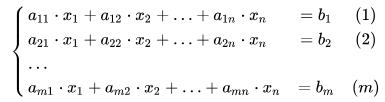
\includegraphics[width=0.5 \textwidth]{1.jpg}
\end{center}

Прямой ход:
\begin{center}
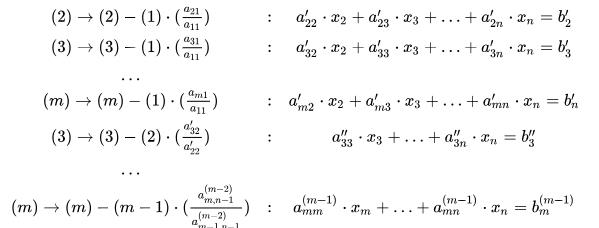
\includegraphics[width=0.7 \textwidth]{2.jpg}
\end{center}

Обратный ход. Из последнего ненулевого уравнения выражаем базисную переменную через небазисные и подставляем в предыдущие уравнения. Повторяя эту процедуру для всех базисных переменных, получаем фундаментальное решение.
\section{Ход работы}
\label{sec:exp}

\subsection{Код приложения}
\label{sec:exp:code}
\begin{verbatim}

#include <iostream>
using namespace std;
void sysout(double **a, double *y, int n)
{
	for (int i = 0; i < n; i++)
	{
		for (int j = 0; j < n; j++)
		{
			cout << a[i][j] << "*x" << j;
			if (j < n - 1)
				cout << " + ";
		}
		cout << " = " << y[i] << endl;
	}
	return;
}
double * gauss(double **a, double *y, int n)
{
	double *x, max;
	int k, index;
	const double eps = 0.00001;  // точность
	x = new double[n];
	k = 0;
	while (k < n)
	{
		// Поиск строки с максимальным a[i][k]
		max = abs(a[k][k]);
		index = k;
		for (int i = k + 1; i < n; i++)
		{
			if (abs(a[i][k]) > max)
			{
				max = abs(a[i][k]);
				index = i;
			}
		}
		// Перестановка строк
		if (max < eps)
		{
			// нет ненулевых диагональных элементов
			cout << "Решение получить невозможно из-за нулевого столбца ";
			cout << index << " матрицы A" << endl;
			return 0;
		}
		for (int j = 0; j < n; j++)
		{
			double temp = a[k][j];
			a[k][j] = a[index][j];
			a[index][j] = temp;
		}
		double temp = y[k];
		y[k] = y[index];
		y[index] = temp;
		// Нормализация уравнений
		for (int i = k; i < n; i++)
		{
			double temp = a[i][k];
			if (abs(temp) < eps) continue; // для нулевого коэффициента пропустить
			for (int j = 0; j < n; j++)
				a[i][j] = a[i][j] / temp;
			y[i] = y[i] / temp;
			if (i == k)  continue; // уравнение не вычитать само из себя
			for (int j = 0; j < n; j++)
				a[i][j] = a[i][j] - a[k][j];
			y[i] = y[i] - y[k];
		}
		k++;
	}
	// обратная подстановка
	for (k = n - 1; k >= 0; k--)
	{
		x[k] = y[k];
		for (int i = 0; i < k; i++)
			y[i] = y[i] - a[i][k] * x[k];
	}
	return x;
}
int main()
{
	double **a, *y, *x;
	int n;
	system("chcp 1251");
	system("cls");
	cout << "Введите ранг матрицы: ";
	cin >> n;
	a = new double*[n];
	y = new double[n];
	for (int i = 0; i < n; i++)
	{
		a[i] = new double[n];
		for (int j = 0; j < n; j++)
		{
			cout << "a[" << i << "][" << j << "]= ";
			cin >> a[i][j];
		}
	}
	for (int i = 0; i < n; i++)
	{
		cout << "y[" << i << "]= ";
		cin >> y[i];
	}
	sysout(a, y, n);
	x = gauss(a, y, n);
	for (int i = 0; i < n; i++)
		cout << "x[" << i << "]=" << x[i] << endl;
	cin.get(); cin.get();
	return 0;
}

\end{verbatim}

\newpage
\section{Работа программы}
\label{sec:picexample}

\begin{figure}[h]
	\centering
	
	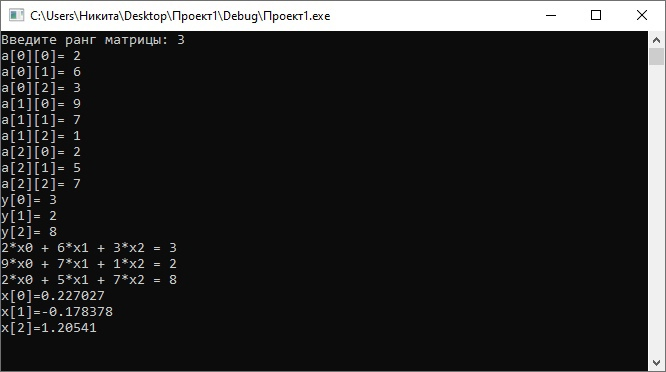
\includegraphics[width=1\textwidth]{prog.jpg}
\end{figure}

\begin{thebibliography}{9}
\bibitem{Knuth-2003}Кнут Д.Э. Всё про \TeX. \newblock --- Москва: Изд. Вильямс, 2003 г. 550~с.
\bibitem{Lvovsky-2003}Львовский С.М. Набор и верстка в системе \LaTeX{}. \newblock --- 3-е издание, исправленное и дополненное, 2003 г.
\bibitem{Vorontsov-2005}Воронцов К.В. \LaTeX{} в примерах 2005 г.
\end{thebibliography}

\end{document}
